\documentclass[border=4pt]{standalone}
\usepackage{tikz}
\usepackage{amssymb}
\usetikzlibrary{shapes.geometric,arrows.meta,positioning,calc}
\usepackage[T1]{fontenc}
\usepackage{helvet}
\renewcommand{\familydefault}{\sfdefault}
\begin{document}
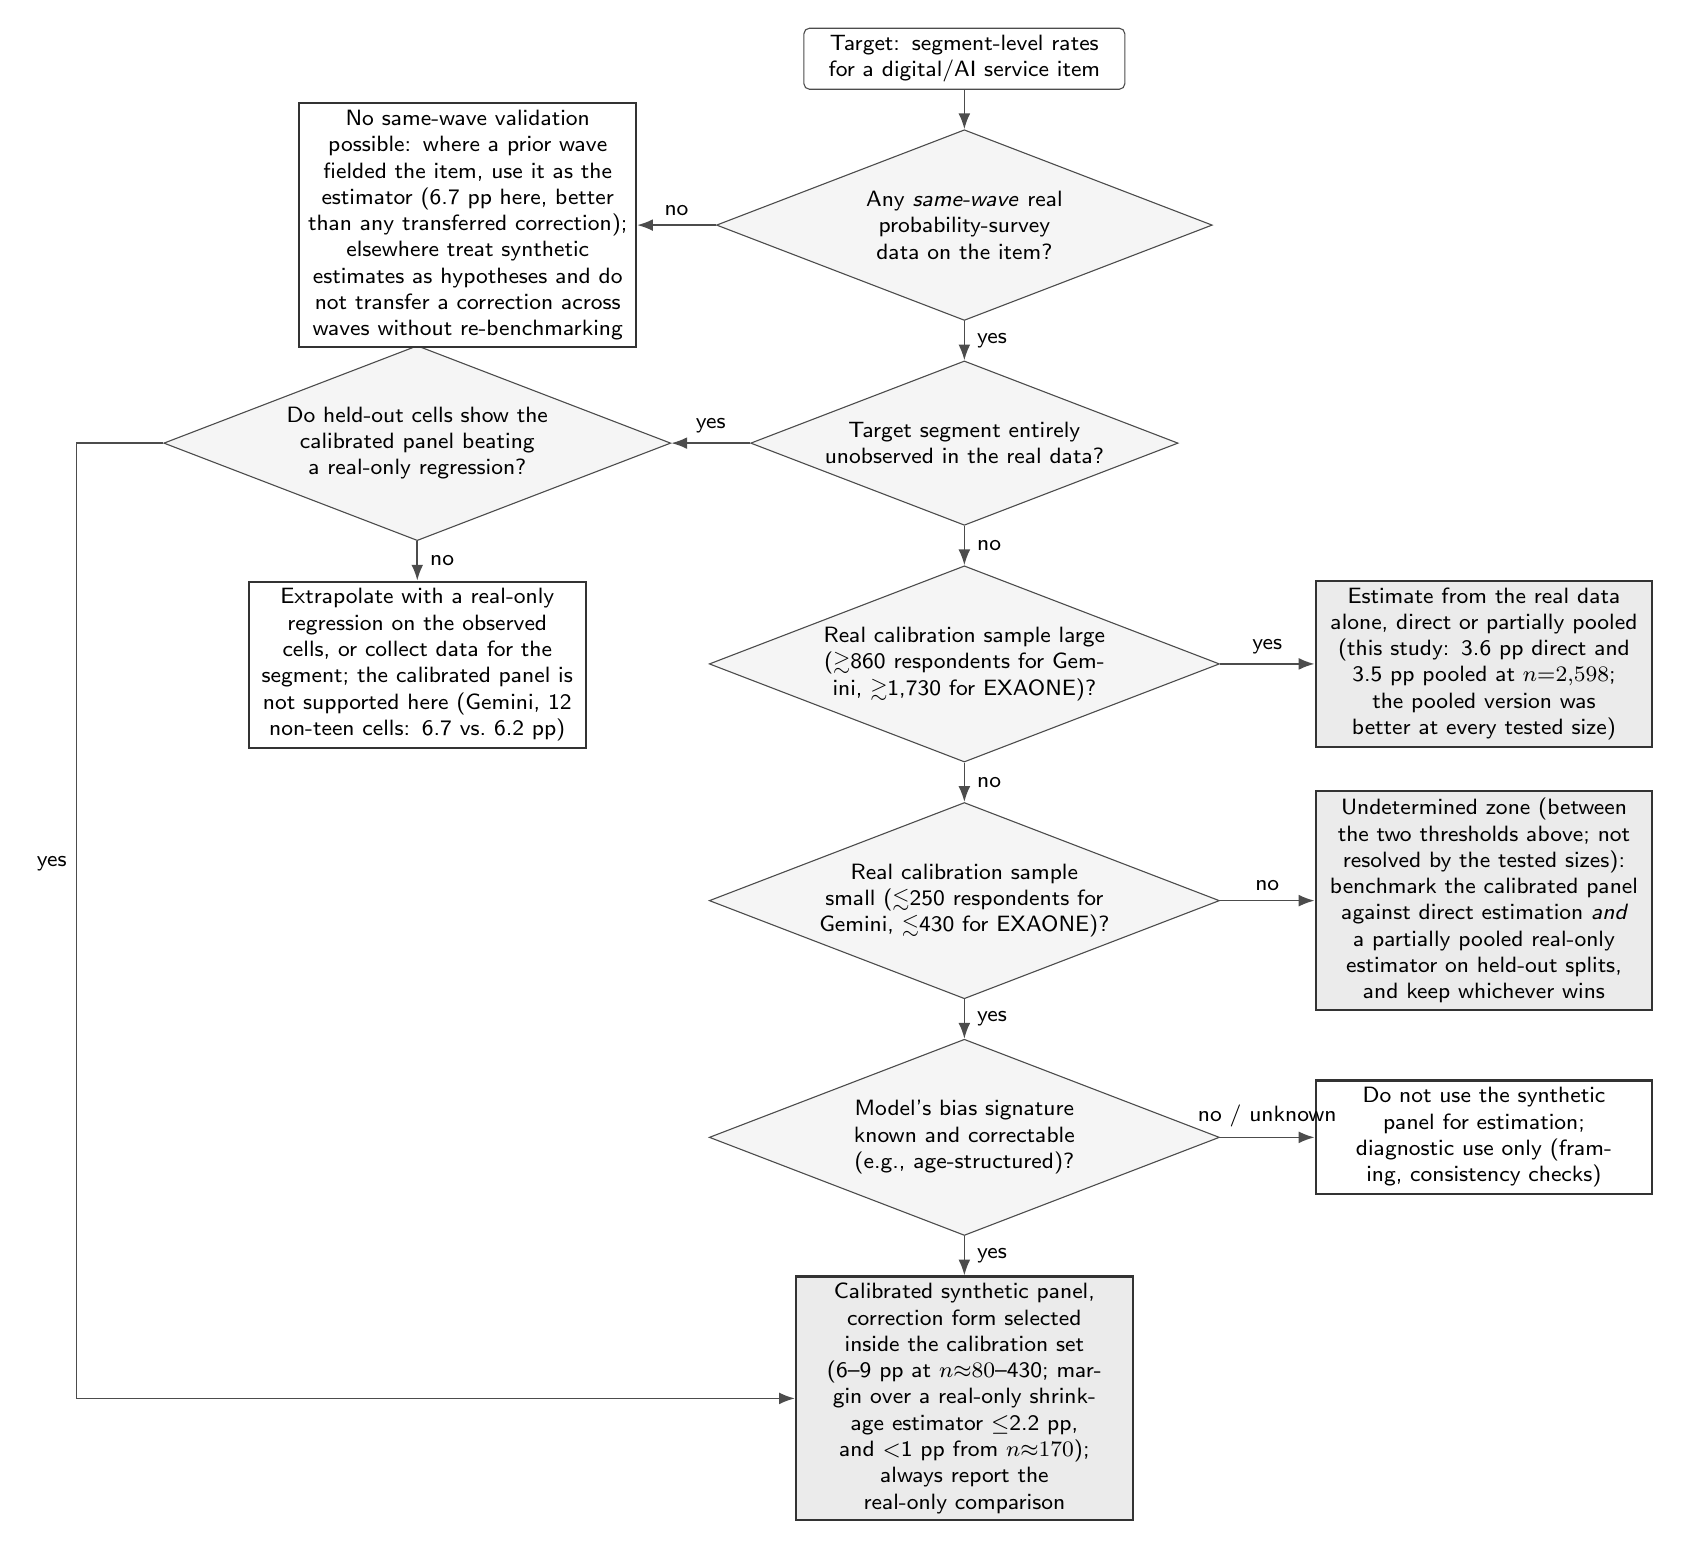
\begin{tikzpicture}[
  font=\footnotesize, node distance=5mm and 6mm, >=Latex,
  box/.style={rectangle,draw=black!70,rounded corners=2pt,fill=white,align=center,minimum height=7mm,inner sep=2.5pt,text width=39mm},
  dec/.style={diamond,draw=black!70,fill=black!4,align=center,aspect=2.6,inner sep=1pt,text width=38mm},
  outb/.style={rectangle,draw=black!80,thick,fill=black!8,align=center,minimum height=8mm,inner sep=2.5pt,text width=41mm},
  warn/.style={rectangle,draw=black!80,thick,fill=white,align=center,minimum height=8mm,inner sep=2.5pt,text width=41mm},
  arr/.style={->,draw=black!70,line width=0.6pt}]
\node[box] (q0) {Target: segment-level rates for a digital/AI service item};
\node[dec, below=of q0] (d1) {Any \emph{same-wave} real probability-survey data on the item?};
\node[dec, below=of d1] (du) {Target segment entirely unobserved in the real data?};
\node[dec, left=of du, xshift=-4mm] (dv) {Do held-out cells show the calibrated panel beating a real-only regression?};
\node[warn, below=of dv] (o5) {Extrapolate with a real-only regression on the observed cells, or collect data for the segment; the calibrated panel is not supported here (Gemini, 12 non-teen cells: 6.7 vs.\ 6.2~pp)};
\node[dec, below=of du] (d2) {Real calibration sample large ($\gtrsim$860 respondents for Gemini, $\gtrsim$1{,}730 for EXAONE)?};
\node[outb, right=of d2, xshift=6mm] (o1) {Estimate from the real data alone, direct or partially pooled\\(this study: 3.6~pp direct and 3.5~pp pooled at $n{=}2{,}598$; the pooled version was better at every tested size)};
\node[dec, below=of d2] (d3) {Real calibration sample small ($\lesssim$250 respondents for Gemini, $\lesssim$430 for EXAONE)?};
\node[outb, right=of d3, xshift=6mm] (o2) {Undetermined zone (between the two thresholds above; not resolved by the tested sizes): benchmark the calibrated panel against direct estimation \emph{and} a partially pooled real-only estimator on held-out splits, and keep whichever wins};
\node[dec, below=of d3] (d4) {Model's bias signature known and correctable\\(e.g., age-structured)?};
\node[warn, right=of d4, xshift=6mm] (o3) {Do not use the synthetic panel for estimation;\\diagnostic use only (framing, consistency checks)};
\node[outb, below=of d4] (o4) {Calibrated synthetic panel, correction form selected inside the calibration set\\(6--9~pp at $n{\approx}80$--430; margin over a real-only shrinkage estimator $\le$2.2~pp, and $<$1~pp from $n{\approx}170$);\\always report the real-only comparison};
\node[warn, left=of d1, xshift=-4mm] (o0) {No same-wave validation possible: where a prior wave fielded the item, use it as the estimator (6.7~pp here, better than any transferred correction); elsewhere treat synthetic estimates as hypotheses and do not transfer a correction across waves without re-benchmarking};
\draw[arr] (q0) -- (d1);
\draw[arr] (d1) -- node[right,xshift=1pt]{yes} (du);
\draw[arr] (du) -- node[right,xshift=1pt]{no} (d2);
\draw[arr] (du) -- node[above]{yes} (dv);
\draw[arr] (dv) -- node[right,xshift=1pt]{no} (o5);
\draw[arr] (dv.west) -- ++(-11mm,0) |- node[pos=0.22,left]{yes} (o4.west);
\draw[arr] (d1) -- node[above]{no} (o0);
\draw[arr] (d2) -- node[above]{yes} (o1);
\draw[arr] (d2) -- node[right,xshift=1pt]{no} (d3);
\draw[arr] (d3) -- node[above]{no} (o2);
\draw[arr] (d3) -- node[right,xshift=1pt]{yes} (d4);
\draw[arr] (d4) -- node[above]{no / unknown} (o3);
\draw[arr] (d4) -- node[right,xshift=1pt]{yes} (o4);
\end{tikzpicture}
\end{document}
